\documentclass[conference]{IEEEtran}
\usepackage[T1]{fontenc}
\usepackage[utf8]{inputenc}
\usepackage{cite}
\usepackage{url}
\usepackage{xcolor}
\usepackage{graphicx}
\usepackage{amsmath}
\usepackage{tikz}
\usepackage{pgfplots}
\pgfplotsset{compat=1.18}

\title{Multi-Protocol Resilient Mesh Gateway for Disaster Communication}

\author{
\IEEEauthorblockN{
Jerald Goh\IEEEauthorrefmark{1},
Amelia\IEEEauthorrefmark{1},
Xuan\IEEEauthorrefmark{2},
Chng Yi Xuan\IEEEauthorrefmark{2}
}
\IEEEauthorblockA{\IEEEauthorrefmark{1}Computing Science, Singapore Institute of Technology}
\IEEEauthorblockA{\IEEEauthorrefmark{2}Information and Communication Technology Cluster, Singapore Institute of Technology}
}

\begin{document}
\maketitle

\begin{abstract}
This project develops a resilient multi-protocol IoT communication gateway for disaster and infrastructure-degraded scenarios where conventional Internet and cellular services may be unavailable or unreliable. The system combines Raspberry Pi Zero 2 W gateways, ESP32 LoRa nodes (LILYGO T3 LoRa32 running Meshtastic), Bluetooth Low Energy (BLE) clients (M5StickC and mobile phones), and WiFi/MQTT clients into a unified architecture that supports cross-protocol message and file exchange. The design enables bidirectional paths such as BLE-to-LoRa-to-WiFi and WiFi-to-LoRa-to-BLE, with real-time routing, topic-based messaging, direct messaging, and chunked file transfer. BLE serves infrastructure-free field access for embedded handheld devices, while WiFi supports multi-user coordination through a browser dashboard — both contributing under 1\% of total end-to-end latency. A latency framework measures BLE RTT, serial RTT, mesh RTT, and derived LoRa RTT, while a web dashboard provides operational visibility through topology, progress reporting, and performance charts.

Implementation emphasizes practical deployment on low-cost hardware using Python services, Flask APIs, MQTT bridging, and systemd orchestration. The gateway degrades gracefully when certain links are unavailable and includes mechanisms to reduce mesh congestion during measurements. Results from prototype integration and functional tests indicate that the architecture is feasible for small multi-hop emergency communication deployments and can support heterogeneous end devices without requiring custom software on every client. The project contributes a deployable, extensible foundation for resilient IoT communication systems and future work in security hardening, autonomous routing policies, and larger-scale performance validation.
\end{abstract}

\section{Introduction, Problem Statement and Objectives}
Natural disasters and emergency situations frequently disrupt conventional communication infrastructure. Cellular towers may be overloaded or offline, and Internet connectivity can become intermittent. In such contexts, there is a need for low-cost, rapidly deployable communication systems that can continue operating in a decentralized fashion. This project addresses that need by designing a multi-protocol mesh gateway architecture where local users can connect through BLE or WiFi, and messages can propagate across LoRa mesh links to remote zones.

The core problem is interoperability under constrained conditions. Existing LoRa mesh deployments often assume homogeneous clients or require users to run specialized software and compatible radio hardware. In contrast, field teams typically carry mixed devices: phones, embedded handhelds, laptops, and ad hoc edge nodes. A practical emergency system must bridge these heterogeneous interfaces while preserving reliability, visibility, and manageable latency.

The proposed solution consists of gateway nodes built on Raspberry Pi Zero 2 W devices connected via USB serial to LILYGO T3 LoRa32 nodes flashed with Meshtastic. Each gateway exposes two local-access channels: BLE Nordic UART Service (NUS) and WiFi with MQTT/web access. Incoming payloads from one interface are normalized and relayed through the LoRa mesh, then republished at destination gateways in the protocol needed by end users. This enables communication paths such as:

\begin{itemize}
\item M5StickC $\rightarrow$ BLE $\rightarrow$ Raspberry Pi $\rightarrow$ serial $\rightarrow$ ESP32 $\rightarrow$ LoRa mesh $\rightarrow$ remote ESP32 $\rightarrow$ serial $\rightarrow$ Raspberry Pi $\rightarrow$ WiFi/MQTT/web
\item Laptop/phone $\rightarrow$ WiFi/MQTT $\rightarrow$ Raspberry Pi $\rightarrow$ LoRa mesh $\rightarrow$ remote gateway $\rightarrow$ BLE notifications
\end{itemize}

The project objectives are:
\begin{enumerate}
\item Build an end-to-end multi-protocol gateway that supports BLE, WiFi/MQTT, and LoRa mesh bridging.
\item Provide topic messaging, direct messaging, and file transfer for field operation.
\item Implement latency observability across communication hops (BLE, serial, mesh, derived LoRa, WiFi).
\item Deliver a deployable and repeatable setup workflow on Raspberry Pi.
\item Demonstrate graceful degradation when one or more links (mesh/BLE/MQTT) are unavailable.
\item Validate functionality through integration and manual field-oriented tests.
\end{enumerate}

The system is designed for resilience rather than throughput maximization. Messages are small, human-centric, and operationally critical. Therefore, architectural emphasis is placed on robust relay behavior, progress visibility, and simple user access.

The architecture was expanded from an initial BLE-to-LoRa relay concept into a dual-channel BLE + WiFi/MQTT gateway, enabling simultaneous heterogeneous access for smartphones, browser clients, and embedded BLE devices. A full hop-by-hop latency measurement chain was added, including automatic progress publication via MQTT and BLE notifications, rather than only basic end-to-end ping checks.

Several additional capabilities were incorporated as the design matured:
\begin{itemize}
    \item \textbf{Chunked file transfer:} The project includes file transfer over the mesh with metadata framing (sender and filename), per-chunk CRC32 validation, and transfer tracking endpoints — supporting payloads up to 50 KB.
    \item \textbf{Gateway status and topology:} Periodic retained MQTT status and compact LoRa status broadcasts enable remote gateway discovery and a live network topology view in the web dashboard.
    \item \textbf{Congestion-aware probing:} Periodic LoRa status broadcasts are paused during mesh latency probing to prevent channel contention from inflating RTT measurements.
    \item \textbf{Automated deployment:} An automated setup pipeline covers AP configuration, MQTT broker setup, BLE stack tuning, and systemd service packaging, reducing manual configuration burden for field deployment.
\end{itemize}

In summary, the project scope evolved from a protocol bridge prototype into a more complete disaster-communications platform with observability, multi-client support, and deployment automation.

\section{Literature Review}
The current state of emergency IoT communication emphasizes resilient low-power wireless links, often using LPWAN technologies (LoRa/LoRaWAN), ad hoc mesh networking, and edge gateways to bridge local user interfaces. Meshtastic-style LoRa mesh systems are attractive in this domain because they support decentralized routing, low power operation, and operation without external infrastructure. At the same time, BLE and WiFi remain the most accessible interfaces for end users carrying commodity devices.

Significant technological developments in this field include:
\begin{enumerate}
\item Mature open-source LoRa mesh firmware stacks (e.g., Meshtastic) that simplify radio-layer routing and peer discovery.
\item Practical BLE service patterns (such as Nordic UART Service) for lightweight message exchange with mobile clients.
\item MQTT-based publish/subscribe middleware for decoupled many-to-many messaging and application integration.
\item Low-cost edge-compute gateways (Raspberry Pi class) that can combine protocol translation, local dashboards, and control logic.
\end{enumerate}

Common methodologies in prior work include simulation-based mesh evaluation, testbed deployment with custom packet formats, and gateway-centric interoperability studies. Performance is typically measured using latency, packet delivery ratio, throughput under contention, and node energy use. These methodologies are effective for benchmarking isolated layers; however, many studies focus narrowly on radio behavior and do not fully evaluate user-facing cross-protocol operation under practical constraints.

Existing approaches show several limitations:
\begin{enumerate}
\item Homogeneous-client assumption: Many systems expect all users to run the same protocol stack.
\item Limited local user integration: Not all designs expose both BLE and browser-friendly interfaces.
\item Insufficient operational observability: Few prototypes provide hop-by-hop latency decomposition for field diagnostics.
\item Fragmented deployment workflows: Reproducibility suffers when setup relies on manual per-device tuning.
\item Security tradeoffs: Rapid prototypes often leave transport-level security and stronger authentication for future phases.
\end{enumerate}

These limitations directly motivate this project. The design objective is not to replace radio research, but to close the gap between communication theory and field-usable, mixed-device operation. By combining BLE NUS, LoRa mesh, and MQTT/web interfaces in one gateway, the project operationalizes interoperability in a constrained deployment. By implementing latency breakdown (BLE/serial/mesh/derived LoRa/WiFi), it aligns measurement with practical troubleshooting needs rather than only aggregate end-to-end timing. By packaging setup scripts and service management, it improves repeatability.

Overall, prior research supports the feasibility of each component layer; this project contributes at the integration layer, where practical disaster communication systems often fail due to interoperability friction rather than radio infeasibility.

\section{Design}
\subsection{Overall Architecture}
The system follows a distributed gateway architecture. Each site has:
\begin{itemize}
\item Raspberry Pi Zero 2 W gateway (application host)
\item LILYGO T3 LoRa32 ESP32 node (Meshtastic mesh endpoint)
\item Local user devices via BLE and/or WiFi
\end{itemize}

Core software modules in the gateway are:
\begin{itemize}
\item \texttt{mesh\_interface}: LoRa-side send/receive via serial (or BLE transport option)
\item \texttt{bt\_server}: BLE NUS peripheral and gateway beacon advertisement
\item \texttt{mqtt\_bridge}: WiFi MQTT bridge and LoRa/MQTT routing logic
\item \texttt{web\_server}: Flask APIs and browser dashboard serving
\item \texttt{latency}: multi-hop RTT probing and aggregation
\item \texttt{file\_transfer}: chunked transfer protocol with CRC32
\item \texttt{message\_store}: thread-safe in-memory message buffer
\end{itemize}

\begin{figure}[t]
\centering
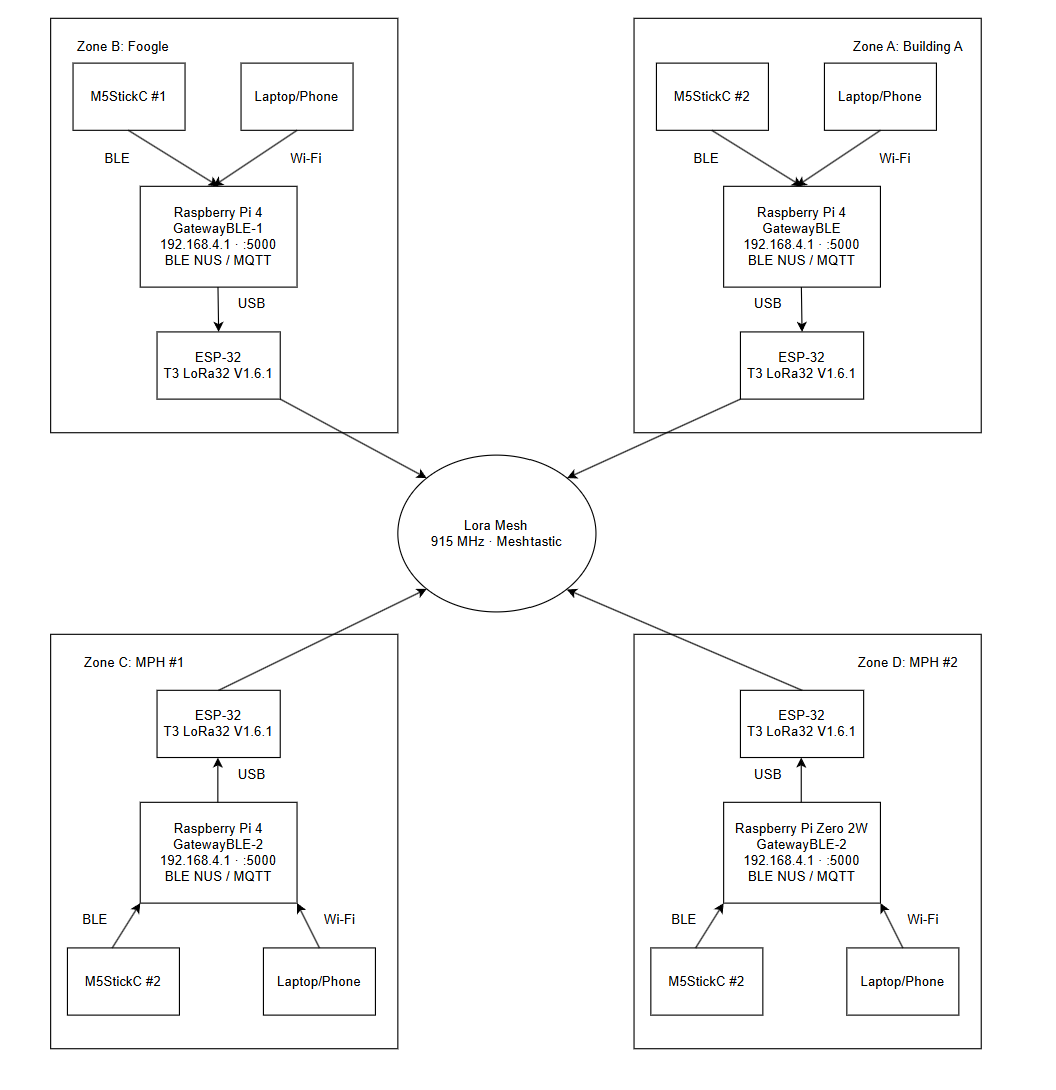
\includegraphics[width=0.48\textwidth]{Diagram_IOT.png}
\caption{System-level architecture showing cross-protocol message flow across BLE, USB Serial, LoRa mesh, and WiFi/MQTT layers.}
\label{fig:architecture}
\end{figure}

\subsection{Device and Sensor/Endpoint Types}
Although the system is message-centric rather than environmental sensing-centric, the effective IoT endpoint classes are:
\begin{itemize}
\item Embedded endpoint: M5StickC Plus BLE handheld client
\item Smartphone endpoint: BLE UART terminal and WiFi browser interface
\item Laptop endpoint: Web UI and MQTT client/CLI tools
\item Mesh endpoint: ESP32 LoRa nodes participating in Meshtastic network
\item Edge compute endpoint: Raspberry Pi gateway node
\end{itemize}

These endpoint classes provide both human-in-the-loop communication and telemetry-style status reporting (latency, node presence, gateway health).

\subsection{Connectivity and Protocol Stack}
Connections and protocols are layered as follows:
\begin{enumerate}
\item End-device local access:
\begin{itemize}
\item BLE NUS (custom gateway advertisement and UART-style write/notify)
\item WiFi AP with local web server and MQTT broker (WebSocket for browsers)
\end{itemize}
\item Gateway-to-radio interface:
\begin{itemize}
\item USB serial to Meshtastic node (primary)
\item Optional BLE transport to radio device in software interface layer
\end{itemize}
\item Inter-gateway/backhaul layer:
\begin{itemize}
\item LoRa mesh via Meshtastic routing
\end{itemize}
\item Application-layer framing:
\begin{itemize}
\item Text wire formats for topic and DM relay
\item Compact gateway status broadcasts
\item Chunked binary transfer frames for file transport
\end{itemize}
\end{enumerate}

\subsection{Data Collection, Storage, and Processing}
Collected data includes:
\begin{itemize}
\item Message content and metadata (sender, timestamp, RSSI, SNR, direction)
\item File transfer metadata and progress
\item Gateway status snapshots (BLE clients, mesh peers, WiFi users)
\item Latency samples (BLE, serial, mesh, derived LoRa)
\end{itemize}

Storage strategy is edge-local, memory-first:
\begin{itemize}
\item Message store: bounded in-memory circular buffer (200 entries)
\item Completed inbound transfers: bounded in-memory cache
\item Latency samples: bounded in-memory arrays
\end{itemize}

Processing includes routing, transformation, and metrics summarization:
\begin{itemize}
\item BLE text to mesh and/or MQTT publish
\item MQTT messages to LoRa wire format
\item LoRa incoming wire parse to topic/DM and MQTT publication
\item RTT summary statistics (last, average, min, max)
\end{itemize}

This approach favors operational responsiveness and simplicity over long-term persistence.

\subsection{User Interaction and Integrations}
Users interact through:
\begin{itemize}
\item BLE device interface (M5StickC display and controls, phone BLE terminal)
\item Browser dashboard for messaging, node view, topology, and latency charts
\item MQTT clients and CLI utility for scriptable chat operations
\end{itemize}

Integration points include:
\begin{itemize}
\item Paho MQTT bridge with local Mosquitto broker
\item Browser MQTT over WebSocket
\item Meshtastic Python interface for LoRa communications
\end{itemize}

The UI includes chat, DM, file transfer notifications, latency tables/charts, and network topology visualization for up to four gateway sites.

\subsection{Security Protocols and Protection Strategy}
Current implemented controls:
\begin{enumerate}
\item WiFi AP uses WPA2-PSK with CCMP.
\item Local MQTT broker binding limits standard MQTT to localhost and WebSocket listener to AP IP.
\item BLE operation is configured for practical reconnect reliability with Just-Works behavior.
\item File transfer integrity uses per-chunk CRC32 checks.
\end{enumerate}

Current limitations:
\begin{enumerate}
\item MQTT allows anonymous clients in current prototype configuration.
\item Web API does not yet enforce token-based authentication.
\item BLE message channel does not include end-to-end encryption at application layer.
\item Message/file payloads are not persistently encrypted in storage (in-memory buffers).
\end{enumerate}

Design review stance: security is partially addressed at link/access configuration level but requires hardening for production deployment (MQTT auth/TLS, API authn/authz, stronger identity management, and cryptographic message protection).

\section{Implementation (Prototype and Testing)}
\subsection{Prototyping Approach and Development Platforms}
The prototype is implemented using:
\begin{itemize}
\item Hardware: Raspberry Pi Zero 2 W, LILYGO T3 LoRa32, M5StickC Plus, smartphones/laptops
\item Firmware/platforms: Meshtastic on ESP32; Arduino framework for M5StickC
\item Gateway software: Python modules for mesh, BLE, MQTT, web APIs, latency, and file transfer
\item Runtime services: Mosquitto broker, hostapd/dnsmasq AP stack, systemd service management
\end{itemize}

The gateway entrypoint wires all components and supports runtime flags to enable BLE, MQTT, and transport settings. This supports progressive bring-up: mesh-only, BLE-only, MQTT-only, or full-stack operation.

\subsection{Deployment Strategy, Challenges, and Mitigation}
Deployment model:
\begin{enumerate}
\item Prepare Pi OS with dependencies.
\item Provision Python virtual environment and project requirements.
\item Configure AP, MQTT broker, BLE behavior, and systemd unit.
\item Connect ESP32 LoRa node by USB serial.
\item Launch gateway service with selected options.
\end{enumerate}

Expected deployment challenges and mitigations:
\begin{enumerate}
\item Hardware dependency failures:
\begin{itemize}
\item Challenge: ESP32 not detected or serial path mismatch.
\item Mitigation: auto-detection workflow and graceful no-hardware mode.
\end{itemize}
\item Wireless coexistence and interference:
\begin{itemize}
\item Challenge: BLE and WiFi contention on constrained radio hardware.
\item Mitigation: disable WiFi power save, tune service behavior, simplify reconnect logic.
\end{itemize}
\item Mesh congestion during active diagnostics:
\begin{itemize}
\item Challenge: periodic status packets can interfere with latency probes.
\item Mitigation: temporary LoRa status broadcast pause during mesh ping sequence.
\end{itemize}
\item Reconnect instability for mobile BLE clients:
\begin{itemize}
\item Challenge: stale bond/state and inconsistent reconnects.
\item Mitigation: BlueZ setup adjustments, stale bond cleanup, beacon-assisted rediscovery, exponential backoff on client.
\end{itemize}
\item Operational setup complexity:
\begin{itemize}
\item Challenge: manual configuration errors.
\item Mitigation: automation scripts and systemd packaging.
\end{itemize}
\end{enumerate}

\subsection{Testing Process for Reliability and Functionality}
Testing is primarily integration and system-level manual testing, including:
\begin{enumerate}
\item Protocol-path validation:
\begin{itemize}
\item BLE $\rightarrow$ LoRa $\rightarrow$ WiFi message path
\item WiFi/MQTT $\rightarrow$ LoRa $\rightarrow$ BLE path
\item Direct message and topic routing behavior
\end{itemize}
\item API and UI verification:
\begin{itemize}
\item Message APIs, transfer endpoints, node discovery, latency endpoints, gateway status
\item Browser dashboard updates via MQTT subscriptions
\end{itemize}
\item File transfer validation:
\begin{itemize}
\item Upload via API, chunk-send sequencing, receiver assembly, CRC mismatch handling
\item Download and metadata correctness checks
\end{itemize}
\item Latency workflow validation:
\begin{itemize}
\item BLE RTT ping from M5StickC
\item Auto-triggered serial + mesh measurements and derived LoRa computation
\item Progress notifications over MQTT and BLE
\end{itemize}
\item Fault/degradation testing:
\begin{itemize}
\item Gateway startup without mesh hardware
\item MQTT unavailable mode
\item BLE-only operation
\end{itemize}
\end{enumerate}

Because this is a design review stage prototype, no formal automated CI test suite is integrated yet.

\subsection{Success Criteria, Metrics, and Benchmarks}
Success is evaluated by functional and performance-oriented criteria:
\begin{enumerate}
\item Functional criteria:
\begin{itemize}
\item End-to-end message relay across mixed protocols is successful.
\item DM/topic semantics are preserved across transport transitions.
\item File transfer reaches completion with integrity checks.
\item Dashboard accurately reflects network and latency state.
\end{itemize}
\item Performance criteria:
\begin{itemize}
\item Measurable RTT per hop (BLE, serial, mesh, derived LoRa).
\item Stable user interaction under small multi-node loads.
\item Bounded memory behavior under sustained messaging.
\end{itemize}
\item Reliability criteria:
\begin{itemize}
\item Reconnect behavior for BLE clients is robust under transient disconnects.
\item System remains operational when optional modules/hardware are absent.
\end{itemize}
\item Deployment criteria:
\begin{itemize}
\item Repeatable setup on Raspberry Pi with minimal manual intervention.
\end{itemize}
\end{enumerate}

Benchmarks are currently comparative and scenario-based (small testbed), with metrics captured from API outputs, logs, and dashboard displays.

\section{Results and Analysis}
\subsection{Scalability and Network Performance Management}
The current system is designed for small-to-medium emergency clusters rather than massive IoT telemetry scale. Scalability controls include:
\begin{enumerate}
\item Bounded in-memory structures for messages and samples.
\item Topic-based decoupling through MQTT for local user fan-out.
\item LoRa payload size checks and compact status encoding.
\item Controlled periodic status intervals and temporary pause during critical probes.
\end{enumerate}

In practical terms, the architecture can accommodate additional local users and nodes up to limits imposed by LoRa duty cycle, channel contention, and edge CPU/network constraints. The gateway's modular design supports horizontal scaling by adding more gateway pairs/zones rather than vertically increasing load on one node.

\subsection{Key Metrics and Observed System Behavior}
Key metrics tracked in the prototype are:
\begin{itemize}
\item Response/latency: BLE RTT, serial RTT, mesh RTT, derived LoRa RTT, WiFi RTT
\item Link quality: RSSI/SNR attached to incoming mesh messages
\item Reliability indicators: ACK tracking for LoRa-forwarded message IDs, reconnect behavior, transfer completion
\item Service availability: gateway status online/offline and peer counts
\end{itemize}

Observed behavior from implementation and manual test flow:
\begin{enumerate}
\item BLE RTT is measurable at user device level and integrated into hop-chain diagnostics.
\item Serial RTT measurement provides a baseline for isolating radio contribution.
\item Mesh RTT can be sampled asynchronously and translated into LoRa estimate.
\item End-to-end message relay works across BLE and WiFi clients through LoRa mesh transitions.
\item File transfer protocol successfully reconstructs payloads when all chunks are received and CRC checks pass.
\end{enumerate}

Table~\ref{tab:latency} summarises the measured per-hop round-trip times collected from the prototype testbed. LoRa RTT is derived rather than directly measured: $\text{LoRa RTT} = \text{Mesh RTT} - 2 \times \text{Serial RTT}_{\text{avg}}$.

\begin{table}[h]
\centering
\caption{Hop-by-Hop Round-Trip Latency — Most Recent Measurement}
\label{tab:latency}
\begin{tabular}{|c|l|r|}
\hline
\textbf{Hop} & \textbf{Path} & \textbf{RTT (ms)} \\
\hline
1 & WiFi (Browser $\leftrightarrow$ RPi)          &     46.00 \\
2 & BLE (M5StickC $\leftrightarrow$ RPi)          &     79.00 \\
3 & Serial (RPi $\leftrightarrow$ ESP32 USB)       &    601.20 \\
4 & Mesh (RPi $\leftrightarrow$ RPi full path)     &  8921.23 \\
5 & LoRa (derived: Mesh $-$ 2$\times$Serial)$^{*}$ &  7804.54 \\
\hline
\multicolumn{3}{l}{$^{*}$Derived, not directly measured.} \\
\end{tabular}
\end{table}

\subsection{WiFi Path vs BLE Path Comparison}

Figure~\ref{fig:pathcomp} shows the end-to-end latency breakdown for both access paths through the mesh. The WiFi path (Browser $\rightarrow$ RPi $\rightarrow$ Serial $\rightarrow$ LoRa $\rightarrow$ Serial $\rightarrow$ RPi $\rightarrow$ destination) totals 9,053 ms, while the BLE path (M5StickC $\rightarrow$ RPi $\rightarrow$ Serial $\rightarrow$ LoRa $\rightarrow$ Serial $\rightarrow$ RPi $\rightarrow$ destination) totals 9,086 ms — a difference of only 33 ms.

\begin{figure}[h]
\centering
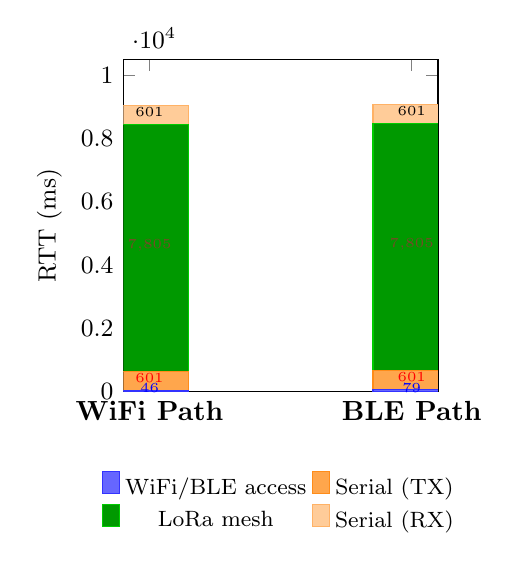
\begin{tikzpicture}
\begin{axis}[
    ybar stacked,
    bar width=28pt,
    width=0.46\textwidth,
    height=5.8cm,
    symbolic x coords={WiFi Path, BLE Path},
    xtick=data,
    ymin=0, ymax=10500,
    ylabel={RTT (ms)},
    ylabel style={font=\small},
    yticklabel style={font=\small},
    xticklabel style={font=\small, font=\bfseries},
    ytick={0,2000,4000,6000,8000,10000},
    legend style={
        at={(0.5,-0.22)},
        anchor=north,
        legend columns=2,
        font=\footnotesize,
        draw=none,
    },
    nodes near coords,
    nodes near coords style={font=\tiny, /pgf/number format/fixed, /pgf/number format/precision=0},
    every node near coord/.append style={yshift=1pt},
]
% Local access hop (WiFi=46, BLE=79)
\addplot+[fill=blue!60, draw=blue!80] coordinates {
    (WiFi Path, 46)
    (BLE Path,  79)
};
% Serial hop 1 (same for both)
\addplot+[fill=orange!70, draw=orange!90] coordinates {
    (WiFi Path, 601)
    (BLE Path,  601)
};
% LoRa hop (same for both)
\addplot+[fill=green!60!black, draw=green!80!black] coordinates {
    (WiFi Path, 7805)
    (BLE Path,  7805)
};
% Serial hop 2 (same for both)
\addplot+[fill=orange!40, draw=orange!60] coordinates {
    (WiFi Path, 601)
    (BLE Path,  601)
};
\legend{WiFi/BLE access, Serial (TX), LoRa mesh, Serial (RX)}
\end{axis}
\end{tikzpicture}
\caption{End-to-end path latency breakdown: WiFi path (9,053 ms) vs BLE path (9,086 ms). LoRa mesh dominates both paths.}
\label{fig:pathcomp}
\end{figure}

The comparison yields a key finding: WiFi and BLE each contribute less than 1\% of total end-to-end latency (0.51\% and 0.87\% respectively), making the two access protocols effectively interchangeable from a latency standpoint. The dominant bottleneck in both paths is the LoRa mesh hop at 7,805 ms, which accounts for 86\% of total path latency. The two serial hops together contribute a further 13\%, leaving the local access protocol as the least significant latency factor. This result supports a key design decision of the system: offering both WiFi and BLE as first-hop options provides broad device compatibility without any meaningful latency tradeoff between them. Device selection can therefore be driven entirely by user preference and hardware availability rather than performance considerations.

\subsubsection{BLE Use Cases in This Project}
BLE is best suited for field personnel operating embedded handheld devices where no pre-existing WiFi infrastructure is available. In this project, BLE serves the M5StickC Plus units carried by field operators. Its primary advantages in this context are:
\begin{itemize}
    \item \textbf{Infrastructure-free access:} BLE requires no WiFi AP association. An M5StickC can discover the nearest gateway via beacon scan and connect directly, making it suitable for rapidly changing field positions.
    \item \textbf{Low power operation:} BLE connection intervals allow embedded devices to remain connected while conserving battery, which is critical for field units in disaster scenarios with limited recharging options.
    \item \textbf{Priority messaging:} The M5StickC client supports emergency presets prefixed with \texttt{!} (e.g., \texttt{!EMERGENCY - Need help}), which are visually flagged across all connected clients.
    \item \textbf{Passive discovery:} The gateway beacon broadcasts mesh status (connected/standalone, client count) in manufacturer data, allowing M5StickC units to select the best available gateway before establishing a connection.
\end{itemize}

\subsubsection{WiFi Use Cases in This Project}
WiFi is best suited for operators or coordinators who are stationary relative to a gateway and carry a laptop, smartphone, or tablet. In this project, WiFi serves browser-based clients and terminal operators via the MQTT web dashboard. Its primary advantages are:
\begin{itemize}
    \item \textbf{Rich user interface:} WiFi clients access the full web dashboard at port 5000, including real-time MQTT chat, network topology visualization, latency charts, file transfer, and gateway status.
    \item \textbf{Multi-user fan-out:} Multiple WiFi clients can connect to the same gateway AP simultaneously and receive all MQTT topic messages, supporting coordination centres with several operators on one gateway.
    \item \textbf{Scriptable access:} The \texttt{mesh\_cli.py} terminal client and REST API allow automated or scripted messaging workflows over WiFi, useful for integration with other emergency management tools.
\end{itemize}

\subsection{Comparison with Similar IoT Solutions}
Compared to single-protocol IoT communication solutions:
\begin{enumerate}
\item Versus pure LoRa mesh clients:
\begin{itemize}
\item Advantage: broader user access (BLE + web + MQTT) without requiring each user to hold a LoRa radio.
\item Tradeoff: increased gateway software complexity.
\end{itemize}
\item Versus LoRaWAN star networks:
\begin{itemize}
\item Advantage: decentralized peer-to-peer resilience without dependence on centralized LoRaWAN infrastructure.
\item Tradeoff: lower coordination and potentially variable latency under contention.
\end{itemize}
\item Versus WiFi-only emergency chat tools:
\begin{itemize}
\item Advantage: extended range/backhaul through LoRa mesh between separated gateways.
\item Tradeoff: lower throughput relative to pure WiFi/IP networks.
\end{itemize}
\end{enumerate}

\subsection{Alignment with Initial Objectives}
Results align strongly with initial project goals:
\begin{enumerate}
\item Multi-protocol bridging objective: achieved.
\item Messaging + file transfer objective: achieved in prototype scope.
\item Latency observability objective: achieved with per-hop decomposition.
\item Deployment repeatability objective: substantially achieved via scripts/systemd.
\end{enumerate}

\section{Conclusion}
This project demonstrates that a low-cost, multi-protocol IoT gateway can provide resilient communication across heterogeneous user devices in infrastructure-constrained environments. The most important outcomes are: (1) successful BLE/WiFi to LoRa mesh interoperability, (2) measured end-to-end path latency of approximately 9 seconds for both access protocols — with LoRa accounting for 86\% — confirming that BLE and WiFi are interchangeable from a performance standpoint and can be selected based purely on device suitability, (3) operationally useful latency decomposition across communication hops, (4) functional chunked file transfer with integrity checks, and (5) deployable service packaging on Raspberry Pi hardware.

The system addresses real-world disaster communication challenges by reducing dependence on conventional network infrastructure and by allowing mixed user devices to communicate through a shared mesh backbone. Its practical value lies in field usability: users can connect through familiar interfaces (phone BLE apps, browser dashboards, MQTT clients) without deep radio expertise.

For the broader IoT field, this work contributes an integration-focused architecture that bridges protocol islands at the edge. It serves as a foundation for more advanced and scalable systems by providing modular components for routing, observability, and user interaction.

Recommended future work includes:
\begin{enumerate}
\item Security hardening: MQTT authentication/TLS, API token-based auth, and stronger identity handling.
\item Reliability upgrades: retransmission strategy for missed file chunks and richer delivery guarantees.
\item Quantitative evaluation: larger multi-site trials with standardized latency/reliability datasets.
\item Scalability optimization: adaptive broadcast intervals and congestion-aware routing policies.
\item Persistence and analytics: optional local database for long-term message/metric retention.
\end{enumerate}

\begin{thebibliography}{99}
\bibitem{meshtastic} Meshtastic Project, ``Meshtastic Documentation,'' [Online]. Available: \url{https://meshtastic.org/}. Accessed: Mar. 30, 2026.

\bibitem{mqtt5} OASIS Standard, ``MQTT Version 5.0,'' Mar. 2019.

\bibitem{btcore} Bluetooth SIG, ``Bluetooth Core Specification,'' [Online]. Available: \url{https://www.bluetooth.com/specifications/}. Accessed: Mar. 30, 2026.

\bibitem{flask} Flask Documentation, ``Flask 3.x Documentation,'' [Online]. Available: \url{https://flask.palletsprojects.com/}. Accessed: Mar. 30, 2026.

\bibitem{mosq} Eclipse Foundation, ``Eclipse Mosquitto MQTT Broker,'' [Online]. Available: \url{https://mosquitto.org/}. Accessed: Mar. 30, 2026.

\bibitem{lora} Semtech Corporation, ``LoRa Modulation Basics,'' Application Note, 2015.

\bibitem{repo} Project Repository, ``IoT2106 Mesh Gateway Source and Setup,'' iot2106, branch feat--bluetooth, 2026.

\bibitem{nus} Nordic Semiconductor, ``Nordic UART Service (NUS) Specification and Usage,'' [Online]. Accessed: Mar. 30, 2026.
\end{thebibliography}

\end{document}
